\chapter{Multiresolution Data and Analysis Methods}
\markboth{Multiresolution Data and Analysis Methods}{}
\label{ch:analysismultires}

%%%%%%%%%%%%%%%%%%%%%%%%%%%%%%%%%%%%%%%%%%%%%%%%%%%%%%%%%%%%%%%%%%%%%%%%%%%%
\begin{fquote}[James Governor] Data matures like wine, and the applications like
fish. \fqsource{{James Governor's Monkchips, 2007}} \end{fquote} 

%%%%%%%%%%%%%%%%%%%%%%%%%%%%%%%%%%%%%%%%%%%%%%%%%%%%%%%%%%%%%%%%%%%%%%%%%%%%

\begin{synopsis}
This chapter describes the application area
and the dataset used in the experiments. The chapter also describes
the usefulness of domain ontology in data analysis; and the  
multiresolution data in the domain of  biology. 
%The chapter also discusses the usefulness of domain ontology in data analysis. 
Finally, the chapter also briefly reviews the 
literature and discusses the related areas of multiresolution 
modelling.
\end{synopsis}

%%          Multiresolution stuff  %%%%%%%%%%%
% copied to previous chapter
%%

Human beings are diploid organisms having two homologous copies of each 
chromosome one each inherited from each parent. 
Copy Number Variations (CNVs) are structural variations in genome
such that a region on the genome will have different copies of 
DNA~\cite{stankiewicz2010}. In human beings, normal copy number 
is two because each child inherits one copy from each parent. Deletion
or loss is the condition when the copy number is less than two. 
Duplication or gain is the condition when the copy number is 
more than two. Similarly, amplification is the condition when 
the copy number increases to more than 5. Some of the cancer 
patients have shown more than hundred copies~\cite{vogelstein2002}.
There are other different kinds of variations but this thesis  
concentrates on copy number aberrations. 

% Nevertheless, during the 
% complex process of cell division, copy number copy numbers could erroneously 
% change from two~\cite{kirsch1993causes}. Such variations in copy numbers are 
% known as copy numbers variation or aberrations. There are other different 
% kinds of variations but this thesis is concentrated in copy number aberration. 
% Deletion, also known as loss, is the situation when the copy number is less 
% than two, i.e. four. Duplication, also known as gains, is the case when the
% copy number is more than two. Similarly, amplification is a special case of 
% duplication when the copy number of the chromosome increases to more than 5.
% Higher level amplifications have been known to increase the copy number to 
% more than hundred fold~\cite{kirsch1993causes}.

%%%%%%%%%%%%%%%%%%%%%%%%%%%%%%%%%%%%%%%%%%%%%%%%%%%%%%%%%%%%%%%%%%%%%%%%%%%%

\section{Chromosomal Aberrations in Cancer}
\label{s:cancer}


Cancer is a heterogeneous collection of diseases characterised 
by abnormal and uncontrolled growth of cells; their ability to 
migrate to other parts of human body and destroy neighbouring cells
and tissues~\cite{bishop99}. Cancer rates have been increasing rapidly
around the globe. Recent World Health Organisation (WHO) report
showed that number of cancer patients escalated to 14.1 million 
in 2012, and  cancer was responsible for 8.2 million deaths in 
2012~\cite{who2014}. 
The menace of cancer is increasing and WHO estimates that cancer 
will  rise by 57\% worldwide in the next 20 years signalling an imminent
human disaster. The cost of cancer is also increasing rapidly. In 2010, 
estimated global cost of cancer reached approximately 963 billion 
euros~\cite{who2014}, which is nine times more than the total 
budgeted expenditure of Finland. 

A wide range of genetic mutations and molecular mechanisms known 
as chromosomal aberrations are identified as the hallmarks
of  disorders such as Cancer, Schizophrenia, and 
infertility~\cite{vogelstein2002}. In cancer research, 
identification and characterisation of chromosomal aberrations 
are crucial for studying and understanding pathogenesis of cancer. 
Moreover, study of chromosomal aberrations provides necessary 
information to select the optimal target for cancer therapy on 
individual level~\cite{kirsch1993causes}. Study of chromosomal 
aberrations also has other clinical applications such as 
studying multiple congenital abnormalities and identifying
the family history of Down syndrome~\cite{obe2007chromosomal}. 



\section{Measurement Technology in Biology}
\label{s:biologymeasure}


\begin{figure}[h!]
\centering
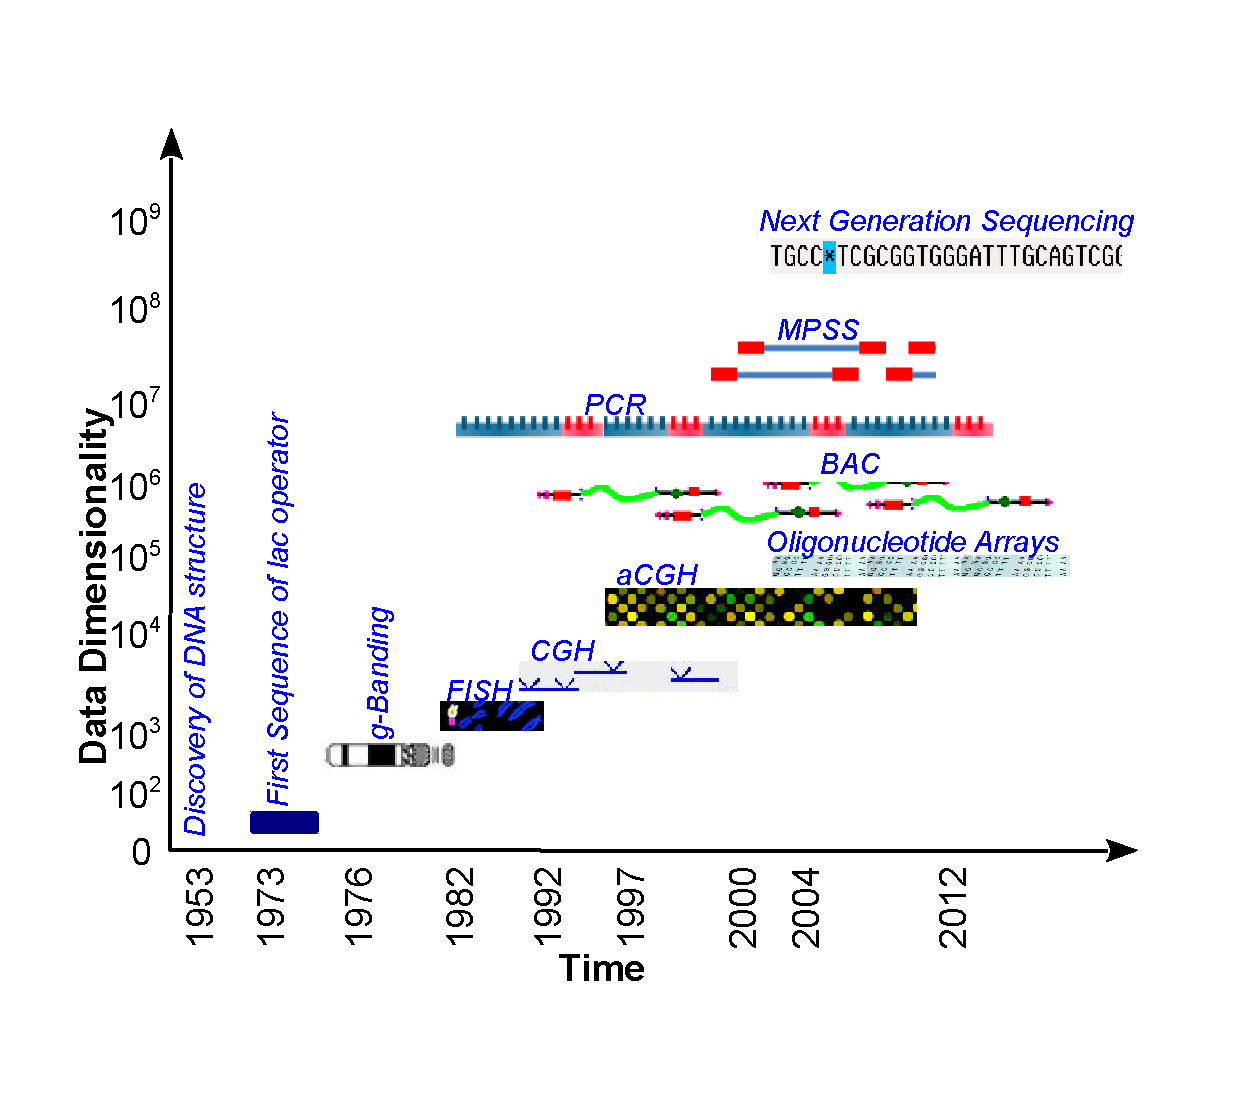
\includegraphics[trim=10mm 20mm 20mm 2mm,width=0.99\textwidth]{figures/arraytypes}
\caption[Evolution of measurement in biology.] {Evolution of measurement technology
in biology described in terms of their level of detail in measurements and time of usage. } 
\label{Fig:arraytypes}
\end{figure}

Years of evolution and adaptation have made organisms complex biological 
beings~\cite{mcshea1991}. Ever improving measurement technologies have also 
provided the facilities to measure the complex phenomena in biology~\cite{united2009new}. 
After the discovery of DNA in 1953~\cite{watson1953dna}, different measurement
methods have been proposed to measure the ge\-nome. First sequence of lac 
operator of 
24 bp was published twenty years after the discovery of DNA in 1973~\cite{gilbert1973nucleotide}. 
Figure~\ref{Fig:arraytypes} summarises the evolution of DNA sequencing
technology from the 1973. Initially, different banding methods such as 
G--banding and Q--banding technologies were developed to produce a visible 
karyotype by staining the chromosomes~\cite{benn1992}. A karyotype here 
denotes the  set of all chromosomes in an organism. Alongside the banding 
technology, FISH (Fluorescence In Situ Hybridisation) was developed to
detect the presence or absence of DNA sequences on chromosomes. Similarly, 
microarray technologies such as the  Comparative Genomic Hybridisation 
(CGH)~\cite{kallioniemi92} and array Comparative Genomic Hybridisation 
(aCGH)~\cite{pinkel98} were developed to study the Copy Number Variations 
(CNV) without requiring culturing of cells. Additionally, Bacterial 
Artificial Chromosome (BAC) was developed to sequence the genomes of 
organisms. 


Similarly, Oligonucleotide arrays that uses oligos of short lengths 
(less than 25 bases) were developed to test large number of oligos 
in presence of smaller number of targets~\cite{lockhart96}. In 
addition, promoter arrays were developed to probe thousands of 
promoter sequences in one array experiment~\cite{wang2005}. 
Besides, Massive Parallel Signature Sequencing (MPSS) was developed
to analyse the level of gene expression by identifying and quantifying 
Messenger Ribonucleic Acid (mRNA) transcripts in the sample~\cite{brenner2000mpss}. 
Likewise, Polymerase Chain Reaction (PCR) were developed to amplify
one or small number of copies of DNA thereby generating large number 
of copies of particular DNA sequences useful for biomedical application
such as DNA sequencing and diagnostic purposes~\cite{pcr2003}.

Around the beginning of this century new technology known as next 
generation sequencing (NGS) had resounding impact in DNA sequencing. 
In~\cite{mardis08} and~\cite{mardis2011}, authors summarise 
the improvement in DNA sequencing which has positive impact on the 
biomedical research providing high throughput and high resolution 
techniques to explore, and answer genomewide biological questions. 
%We have only shown two next generation sequencers in the Figure~\ref{Fig:arraytypes}. 
%Nevertheless, different vendors have produced different sequencers
%for commercial use~\cite{liu2012}.
The Carlson curve accurately predicted the doubling time of DNA sequencing 
technologies measured in terms of cost and performance~\cite{carlson2003}.
Furthermore, the curve illustrates the dramatic decrease in cost which is 
sometimes hyperexponential and similar dramatic improvements in technology
to measure biological phenomenon such as DNA sequencing and synthesis, 
gene expressions, and protein structures.

These improvement in measurement technology in biology over the 
period of time produces data in different representation. 
Consequently, multiresolution data are also present 
in biology. For example, measurements from an older generation
technology (eg. G--banding) can be represented in data with
dimensionality in hundreds~\cite{benn1992,shaffer05}. 
In contrast, newer generation technology such as 
microarray measures the same karyotype generating the
data of dimensionality of thousands~\cite{kallioniemi92,pinkel98}. 
In addition, latest technology known as Next Generation Sequencing 
produces the data with millions of dimensions~\cite{mardis08,roh10com}.

The Figure~\ref{Fig:arraytypes} shows major changes in
sequencing technology. However, within each generation of technology
there are several minor improvements.  For example, aCGH 
improves the mapping resolution of 20Mbp (Megabase Pairs) to 100 
Kbp (Kilobase Pairs) over its predecessor CGH.
Similar methods within a generation of technology  also produce
data in different resolutions because  of improvements within 
the technology such as microarrays and banding. For example, authors 
in~\cite{usvasalo2010} use microarray data in two resolutions of 
44000 and 244000 measurements per microarray measured by Agilent 
44B and 244A aCGH platforms to classify different types of leukemias.
Similarly, in NGS, different vendors have produced different sequencers
for commercial use~\cite{liu2012}.

Studying the data generated by different technologies above produces 
wide range of benefits, especially in understanding of the biological
phenomenon. Therefore, computational methods have been used 
to analyse the generated data. The phenomenon of doubling of 
number of transistors in a chip within 18 to 24 months, often known as 
Moore's Law~\cite{moore1965}, has improved the processing power of 
computers exponentially. Similarly, with the advent of Internet and 
other communication technologies and protocols; communication systems
have also improved dramatically. The data storage capacity is also
rapidly rising. These  advancements have resulted in  improved 
computing power thus facilitating development of novel algorithms
to analyse the generated data.

\subsection*{Pan--cancer Analysis}
\label{ss:pancancer}

In addition to the data in different resolutions, efforts have 
been made to study different cancer types by collecting data from 
different sources in pan--cancer  initiative~\cite{pancancer}. 
The aim of the study is to develop an integrated picture of
commonalities, differences, and emergent themes across tumour 
lineages. The initiative involves multiple datasets and 
multiple cancers showing possible utility of multiresolution methods 
in pan--cancer initiative. In the previous
research of our research group, we have considered all cancers 
within a single analysis~\cite{myllykangas06}.



\section{Multiresolution Chromosomal Amplification Data}
\label{s:multchrdata}

Similar to the array technology and next generation sequencing, 
the International System for human Cytogenetic Nomenclature (ISCN)
has defined five different resolutions of the chromosome namely:
300, 400, 550, 700, and 850 in G--banding~\cite{shaffer05}. Each resolution 
defines the precision in division of karyotype. 
For example, in coarse resolution, a karyotype is divided into 
312 ($\approx 300$) different regions, i.e., with lower precision.
In contrast, in fine resolution, a karyotype is divided into 862
($\approx 850$) different regions, i.e., with higher precision
compared to resolution 300.


%%%%%%%%%%%%%%%%%%%%%%%%%%%%%%%%%%%%%%%%%%%%%%%%%%%%%%%%%%%%%%
%%%%%%%%%%%%%%%% chromosome 21 figure drawn goes here %%%%%%%%


\begin{figure}[h!]
\centering
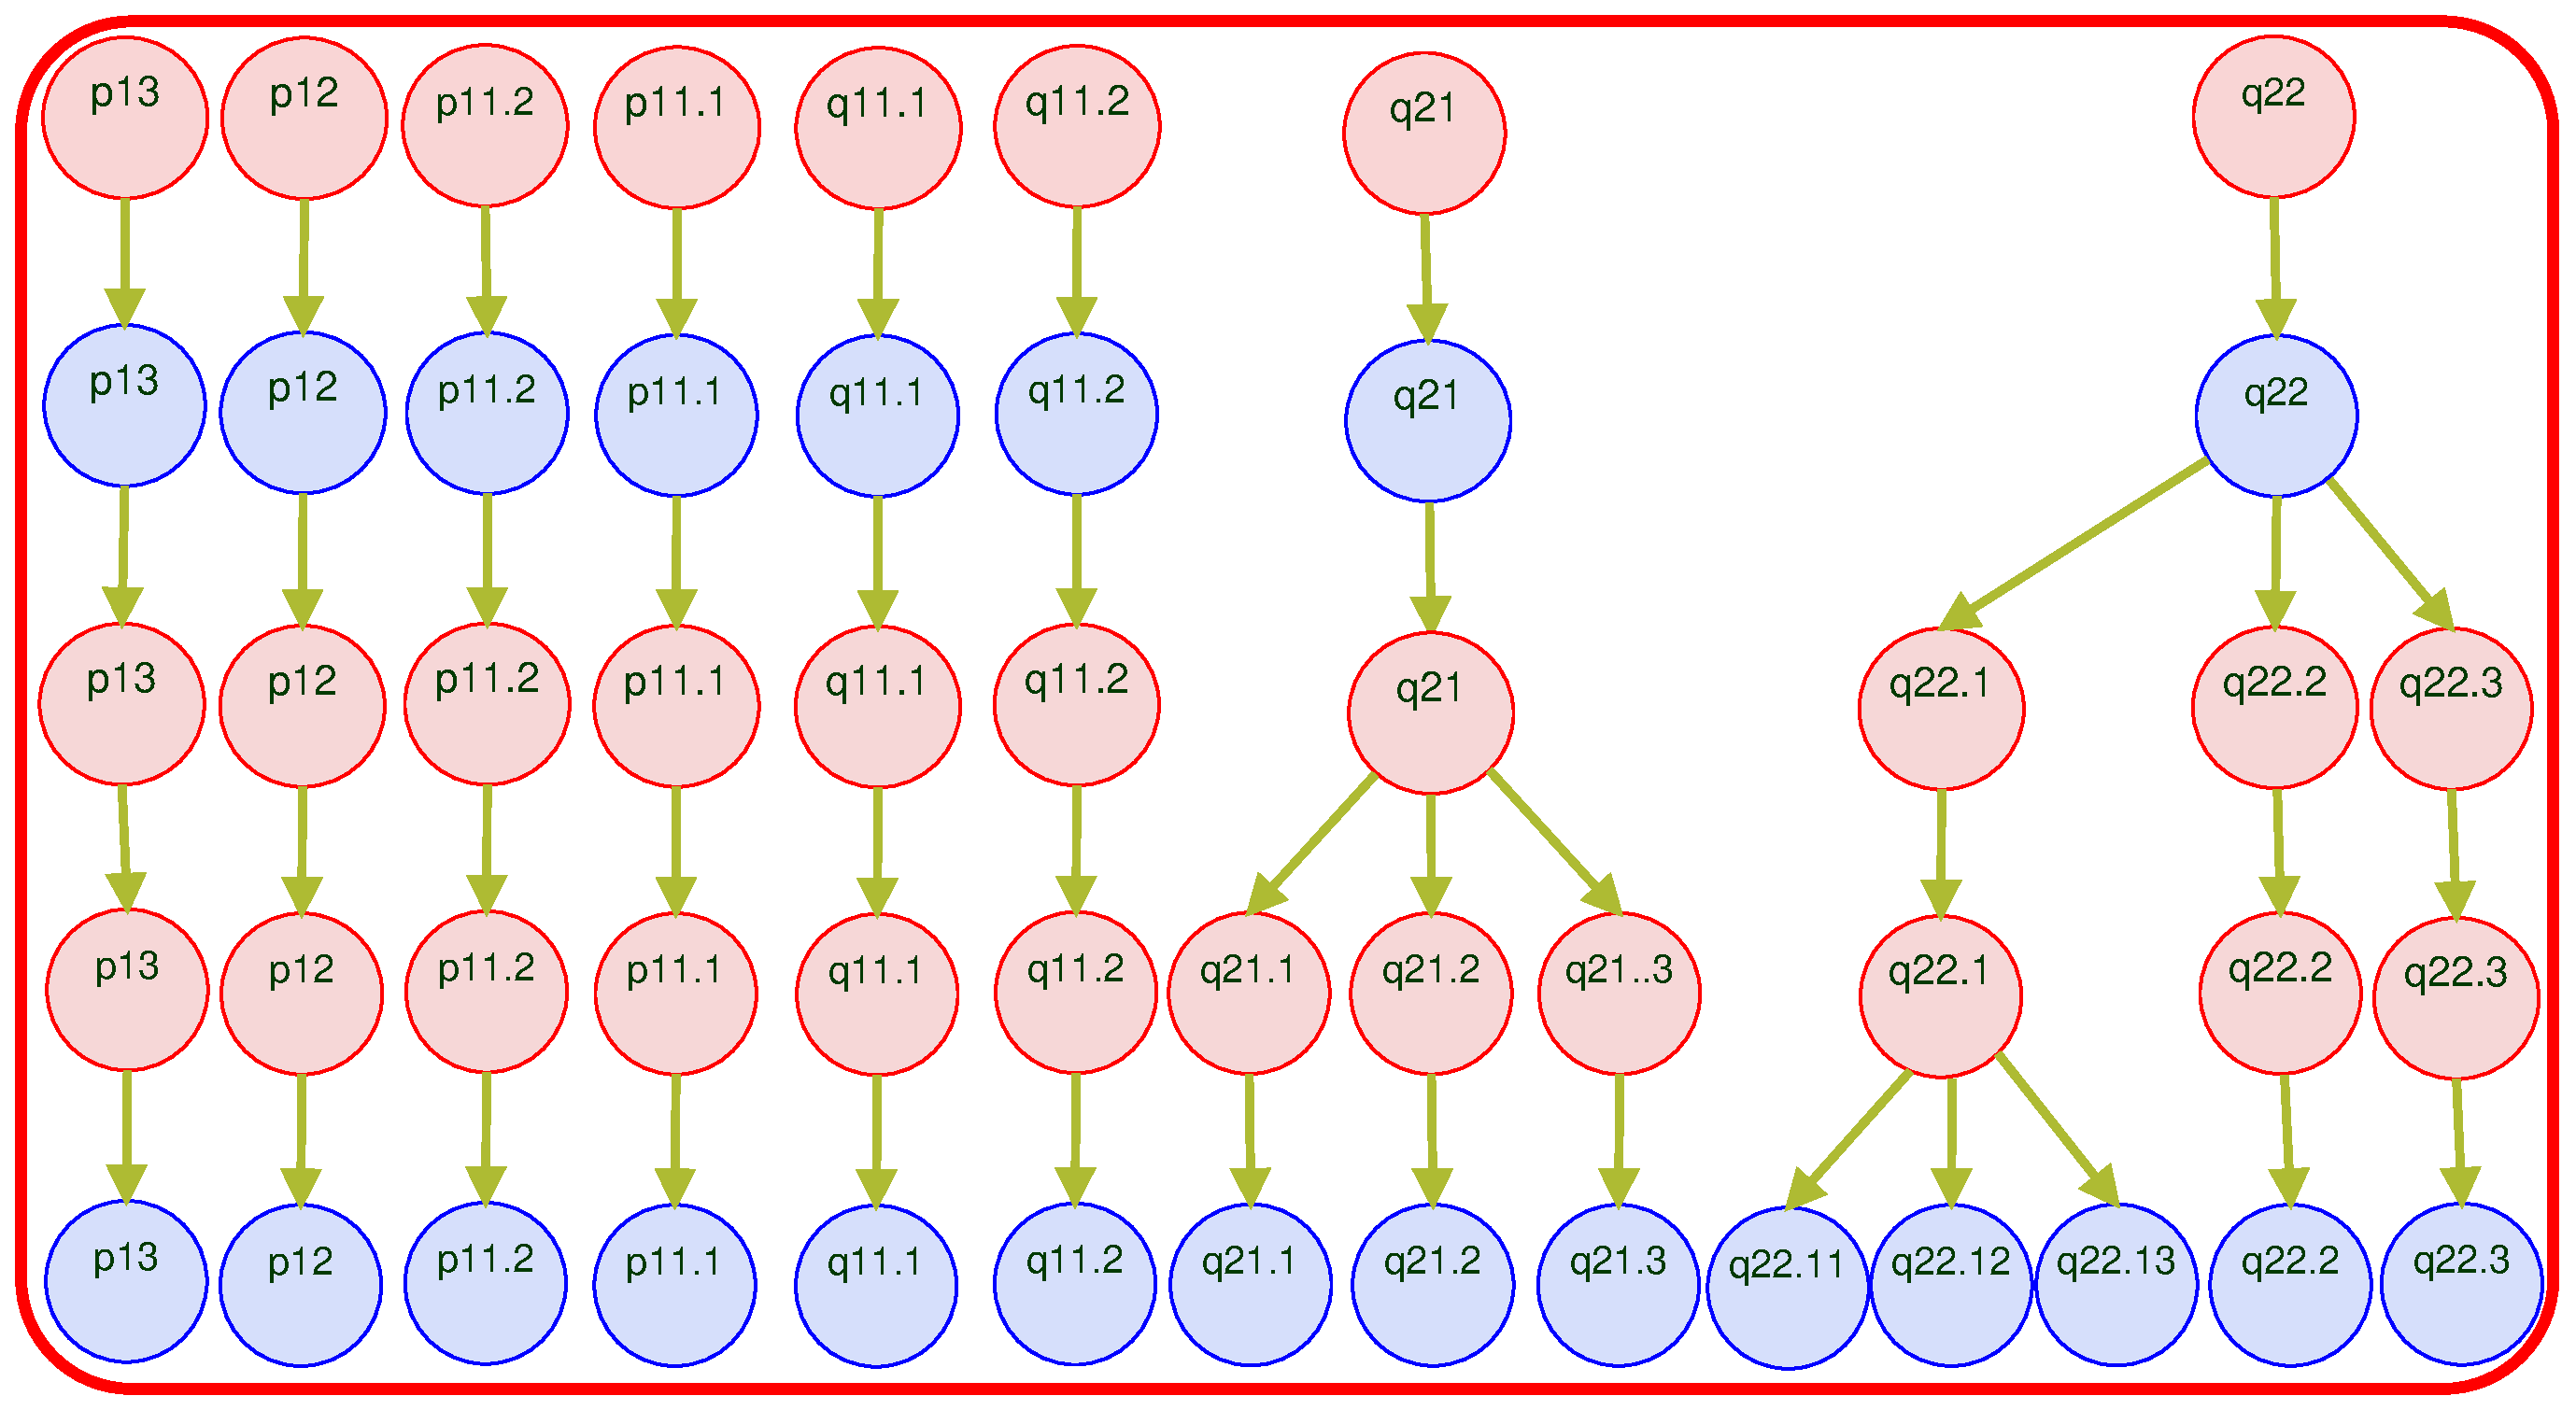
\includegraphics[trim=10mm 5mm 20mm 0mm,width=0.99\textwidth]{figures/chain}
\caption[Multiple Resolutions of the Genome.]{A typical 
relationship between multiple resolutions of genome.  
Figure shows chromosome 21 in five different resolutions 
of genome as defined by ISCN standard. The division is irregular,
and hierarchical but consistent because of the ISCN standard.
Chromosome 21 is chosen for the clarity of the presentation 
because it is the smallest chromosome. Y--axis denotes different resolutions
of genome while x--axis denotes spatial coordinates (different regions) of the genome.
Figure is adapted from~\citepub{c3}.} 
\label{Fig:chr21}
\end{figure}


%%%%%%%%%%%%%%%%%%%%%%%%%%%%%%%%%%%%%%%%%%%%%%%%%%%%%%%%%%%%%%

Figure~\ref{Fig:chr21} shows five different resolutions in 
chromosome 21 according to the ISCN standard. The figure depicts 
the division of regions and chromosome nomenclature with 
an example in chromosome 21. Chromosome 21 is chosen 
for visualisation because it is the smallest chromosome. Chromosome 21 is
divided into 8, 8, 10, 12, and 14 regions in resolution
300, 400, 550, 700, and 850. The nomenclature of the regions 
and their division in different resolutions are irregular 
and hierarchical~\cite{shaffer05}. Some regions are  
undivided whereas other regions are divided into  
different number of regions. For example, the regions 21p12 and 
21p13 are undivided in all the resolutions where as the 
region 21q22 is  divided into 3 and 5 different regions 
in resolution  550 and 850. This division of karyotype
in different levels of detail allows 
measurement technologies to generate data in multiple
resolutions. Each chromosomal region in coarse 
resolution is related with a chromosomal region in
fine resolution with a one to many relationship. 
Given the measurements of same subject in two different
resolutions, the aberrations should be consistent with
each other, i.e., the aberrations should be the same except for some 
measurement errors.

%%%%%%%%%%%%%%%%%%%%%%%%%%%%%%%%%%%%%%%%%%%%%%%%%%%%%%%%%

%data21multi
\begin{figure}[h!]
\centering
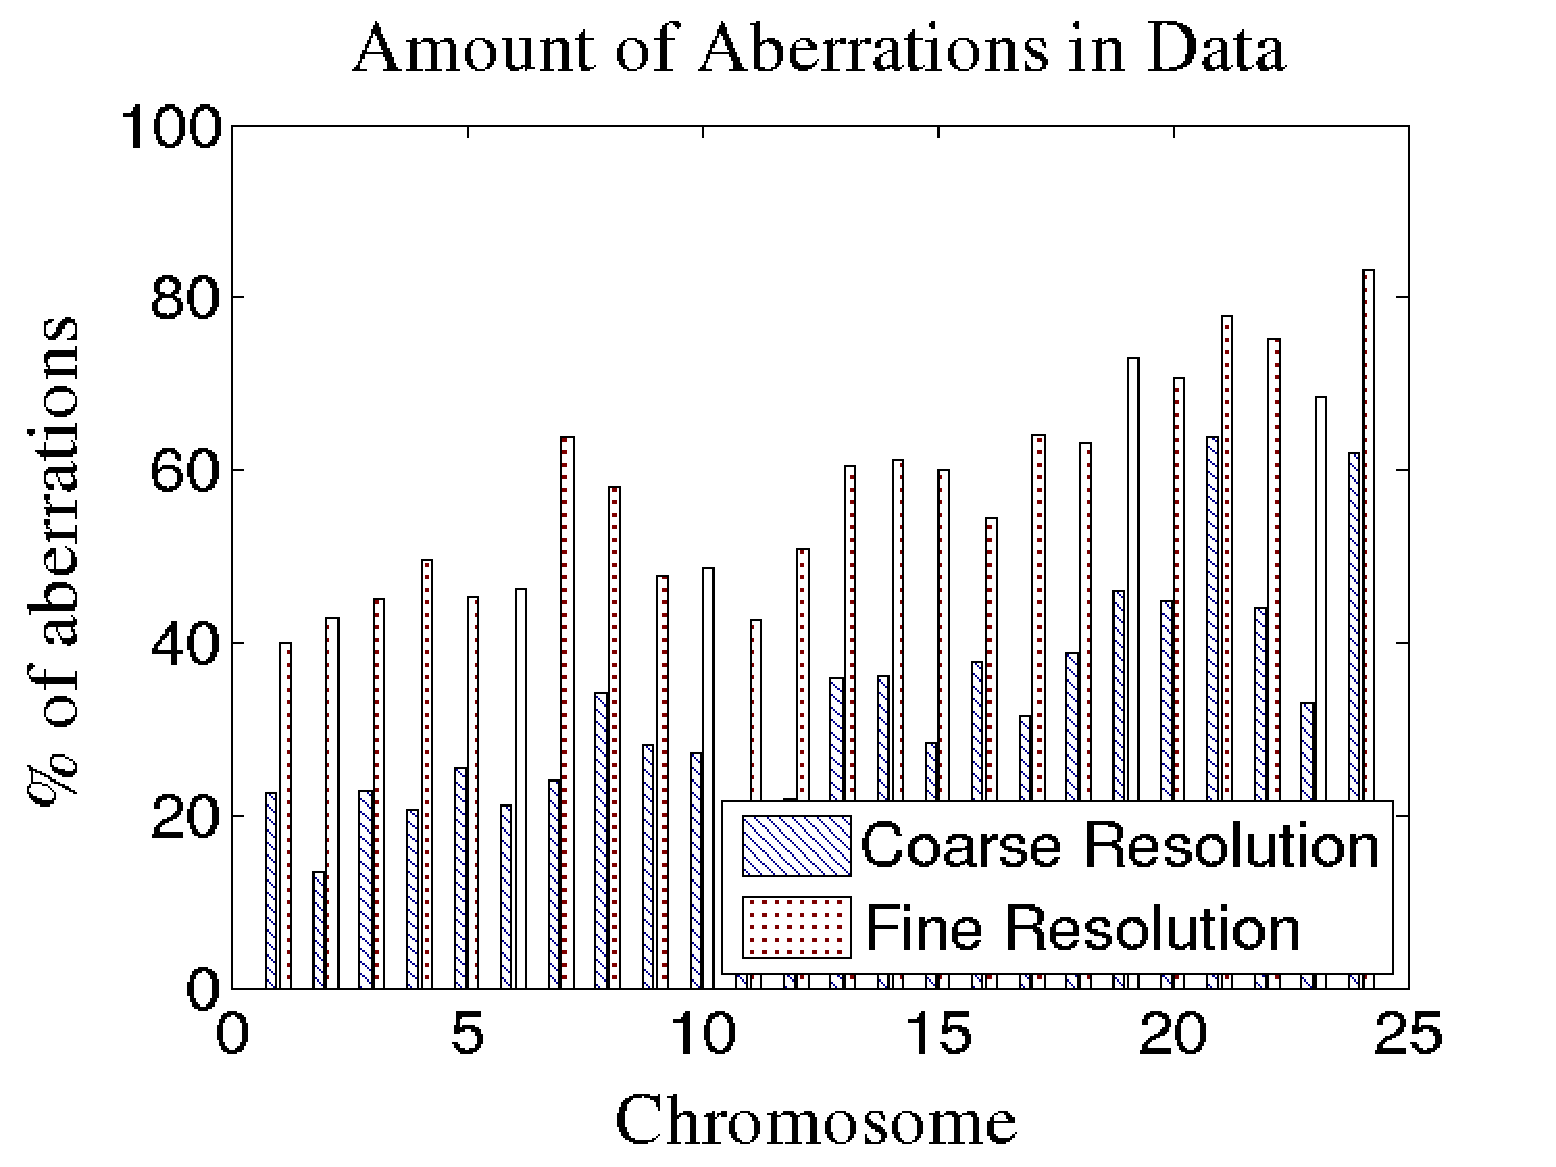
\includegraphics[trim=5mm 2mm 18mm 2mm,width=0.99\textwidth]{figures/perabar}
\caption[Amount of Aberrations in Different Chromosomes]
{Amount of aberrations in each chromosome in two datasets in different data
resolutions. The bar diagram shows that chromosomes in fine resolution 
are comparatively more aberrated than the coarse resolution.} 
\label{Fig:perabar}
\end{figure}


%%%%%%%%%%%%%%%%%%%%%%%%%%%%%%%%%%%%%%%%%%%%%%%%%%%%%%%%%%%%%%%%%%%%%%%%%%%%%

For the experiments, two different datasets were available
in coarse resolution and fine resolution. Researchers at 
the University of Helsinki compiled a dataset of chromosomal 
amplification in coarse resolution reading through the 
literature published between 1992--2002~\cite{knuutila2000}. 
All 838 journal articles were read through manually.
The data describes the chromosomal amplification patterns of 
4590 cancer patients in coarse resolution, i.e., resolution 
400 where a karyotype is divided into 393 different regions.
Similarly, data in fine resolution extracted 
from~\cite{progenetix,baudis07} describes chromosomal
amplification in fine resolution, i.e., resolution 850 where
a karyotype is divided into 862 different regions. Since the 
cancer patients were not the same, there is no direct 
correspondence between data samples in two different 
resolutions. Therefore, most of the analysis methods 
discussed in this thesis consider unsupervised methods
which learn the hidden structure in the data without the 
help of the class labels~\cite{bishop06,mitchell97}.
If the measurements were available from the same cancer patients
in two different resolutions, we can expect consistent matching 
in aberrations except for measurement errors.

In the coarse resolution data, a total of 26527 (out of 1,803,870) matrix elements
are aberrated which accounts for approximately 1.5\% of the total matrix 
elements in the dataset. In all our experiments, we  process 
the data chromosomewise to reduce the data dimensionality and 
with the expectation of finding chromosome specific patterns 
to describe different cancers. When the data is divided into 
each chromosome, there are some samples which do not show 
aberration in any of the chromosomal regions. Such data samples
are deleted as we are interested in modelling chromosomal aberration
patterns and their relation to cancer, not their absence.
Therefore, number of samples and data dimensionality
in each chromosome is different. We therefore calculate percentage
of aberrations in each chromosome in each resolution for comparison purposes. Figure~\ref{Fig:perabar} 
depicts the amount of aberrations in both coarse resolution 
and fine resolution data. Data in fine resolution shows more 
aberration than the data in the coarse resolution. The percentage 
of aberrations are approximately 50\% overall, while the minimum 
and maximum are approximately 15\% and 80\% respectively.



\begin{figure}[h!]
\centering
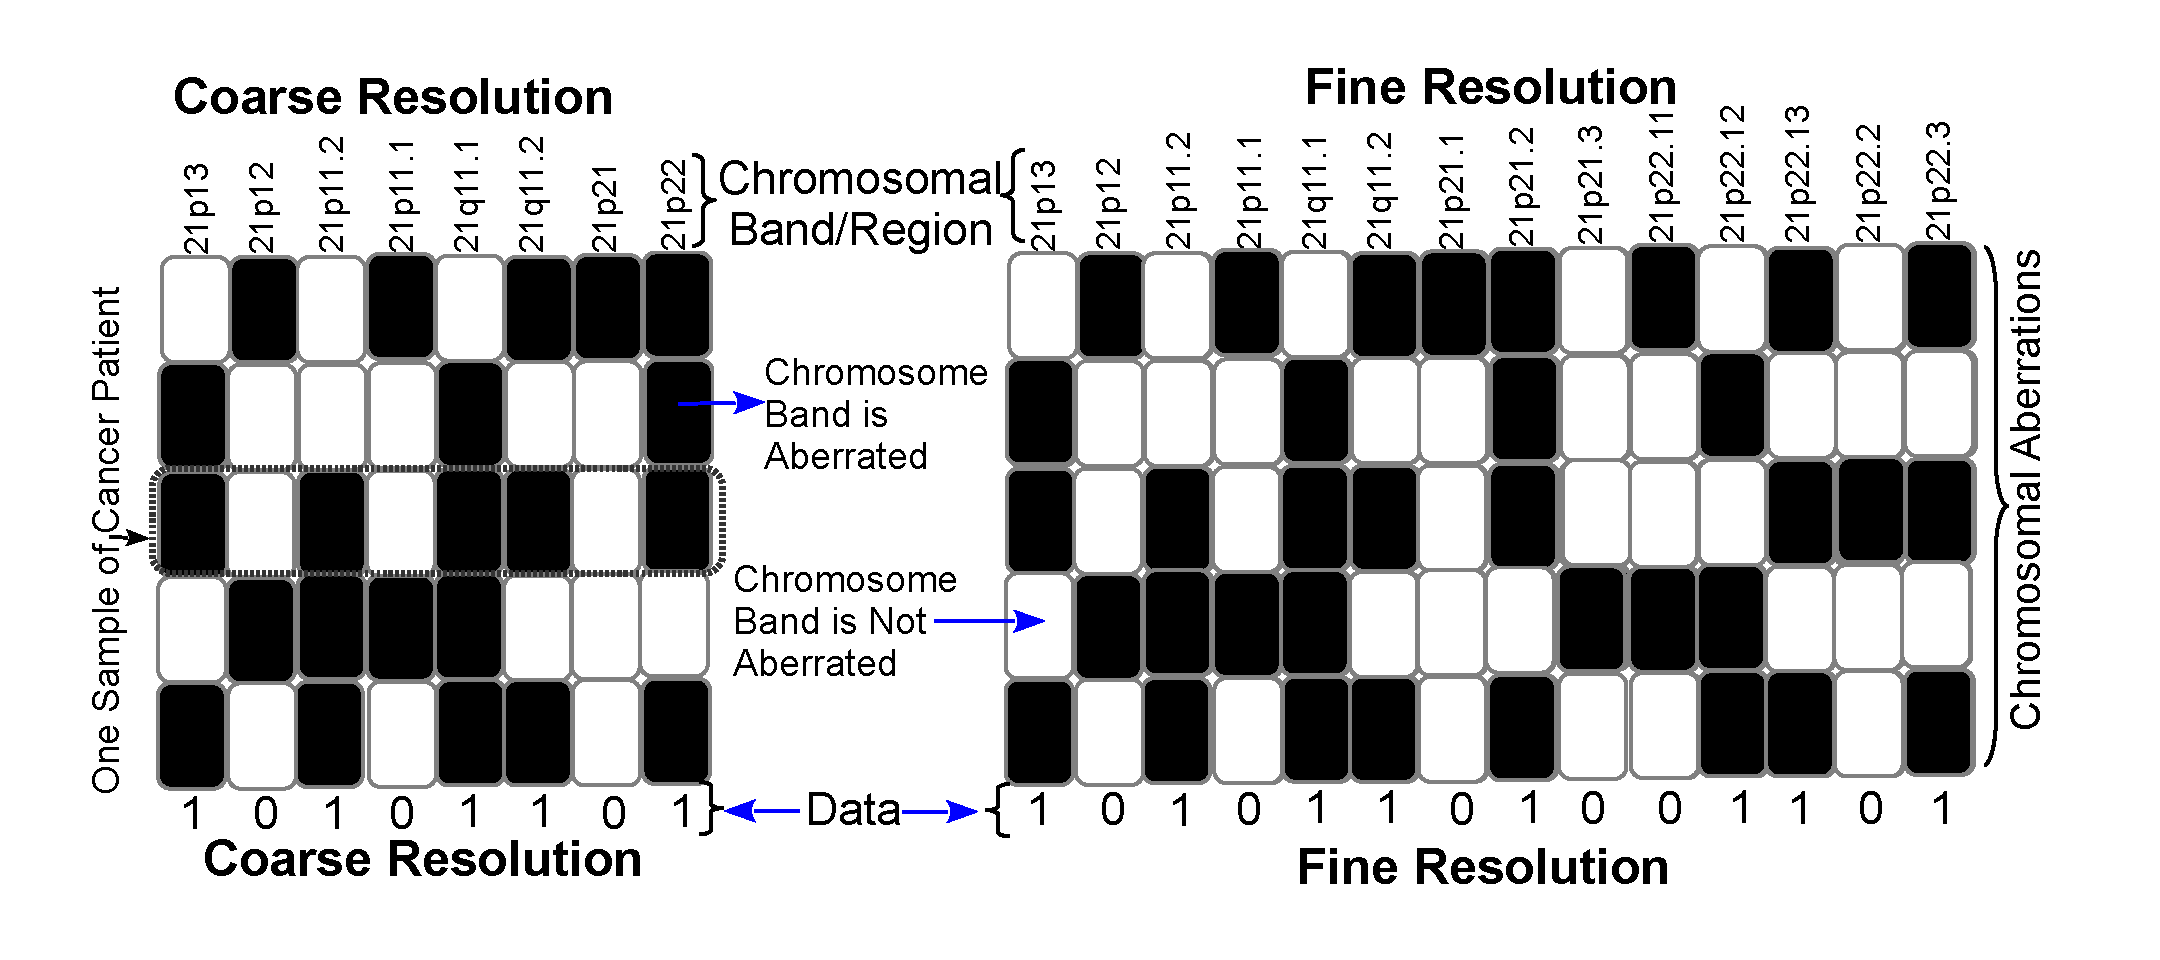
\includegraphics[trim=10mm 10mm 20mm 2mm,width=0.99\textwidth]{figures/data21multi}
\caption[Multiple Resolution in Chromosome 21.]
{Visualisations of data describing chromosome 21 in two different 
resolutions: 300, and 850. Each sample, i.e., each row denotes one 
cancer patient and each column determines a chromosomal region. 
The black colour denotes presence of amplification and white col or 
denotes the absence of amplification. The two different panels in 
the figure depict the same phenomenon measured at different resolutions.
Some chromosomal regions (variables or features in machine learning 
terms) such as 21p21 in left panel have been divided into different 
regions such as 21p21.1, 21p21.2, and 21p21.3 in the right panel. 
Figure is adapted from~\citepub{j1}.} 
\label{Fig:datamulti}
\end{figure}

%%%%%%%%%%%%%%%%%%%%%%%%%%%%%%%%%%%%%%%%%%%%%%%%%%%%%%%%%%%%%%%%%%%%%%%%%%%%%

Figure~\ref{Fig:datamulti} depicts five samples of data from 
chromosome 21 in both the coarse and the fine resolution.
In the Figure~\ref{Fig:datamulti}, rows denote the cancer patients 
and the spatial coordinates on the X--axis denote the chromosomal 
region.  In addition, white colour denotes value of zero (0), i.e.,
the absence of amplification, and  black colour denotes the value 
of one (1), i.e., amplification in that specific region of genome 
for that specific cancer patient. The left panel of the  
Figure~\ref{Fig:datamulti} shows that one region 21p21 in coarse 
resolution is divided into 3 regions in the fine resolution:  
21p21.1, 21p21.2, and 21p21.3 as shown in the right panel of the
figure. In contrast, some of the regions such as 21p13 and 21p12 
are same in both coarse and fine resolution. 
%Therefore, different regions are divided differently. 
Some regions are undivided while other
regions are divided into varying number of regions. Nevertheless, 
the division is consistent because of the ISCN standard. Detailed 
description of the amplification dataset in coarse resolution 
can be found  in~\cite{myllykangas06}.








%%%%%%%%%%%%%%%%%%%%%%%%%%%%%%%%%%%%%%%%%%%%%%%%%%%%%%%%

\section{Ontology of Multiresolution Data}
\label{s:ontologymulti}

The concept of ontology transcends back to the dates of noble 
philosophers Aristotle, Parmenides, and Jacob Lorhard, who 
used the term ontology in the philosophical context to
describe the state of being, and reality~\cite{cohen2014}.
Recently, the term ontology has found its prominence 
in computer and information science community. 
In computer science community, ontology is 
the mechanism for explicit description of the 
conceptualisation of the knowledge represented in the 
knowledge base~\cite{gruber1993,swartout1996}. 

Ontology is a popular methodology to describe the semantics of the 
data in machine learning and data mining community~\cite{panov2012}. 
Recent studies have shown that relevant additional knowledge enhances 
the knowledge discovery process of empirical data~\cite{panov2012}. 
Expansion of semantic web and increasing 
availability of domain knowledge as  ontologies has resulted
in  growth of semantic data. Semantic data mining algorithms
address the challenge of mining abundance of knowledge 
encoded in domain ontologies constrained by the heuristics 
computed from the empirical data~\cite{Vavpetic13jiis}. 

Multiresolution data conceptualises one of the essential 
ontological dichotomies of universals and particulars
in metaphysics~\cite{so49866,russell1911}. The data
in the coarse resolution can be conceptualised as 
universals whereas data in fine resolution can be 
conceptualised as particulars. Therefore, we 
can use ontological information in modelling 
multiresolution data as in~\citepub{c3} and \citepub{j2}.

Biological systems are complex consisting of many interwoven subsystems that 
effect the functionalities of each other~\cite{kim2003}. As a result, 
chromosomal amplifications can effect, and be effected by other 
biological phenomenon. Furthermore, cancer is a multifactorial 
disease and the heterogeneity of cancer also suggests that biological 
phenomenon besides chromosomal aberration can catalyse the development
of cancer. For this reason, additional background knowledge in biology 
was used to enhance the comprehensive analysis of chromosomal 
amplification datasets and to help understand the phenomenon of cancer. 
The additional knowledge used in the analysis of multiresolution data 
are the taxonomy of hierarchy of chromosomal regions, the cancer genes,  virus 
integration sites, fragile sites, and ampli\-fication hotspots
in~\citepub{j2}. Only taxonomy of hierarchy of regions is used
as background ontology in~\citepub{c3}.

The mutations in genes resulting to a larger extent by ``acquired 
mutation'' and to a lesser extent by ``germline mutation'', known 
as cancer genes, are one of the most prominent causes of 
cancer~\cite{futreal2004}. Authors in~\cite{futreal2004} have 
listed the cancer genes and compared them to the complete gene
set revealed by the human genome sequence. Similarly, fragile 
sites are nonrandomly distributed loci on human  chromosome 
that show a constriction or a gap and increased frequency of 
chromosome breakage under the conditions of partial 
replication stress~\cite{durkin07,schwartz06}. The fragile 
sites are often found rearranged in cancers~\cite{glover2005}. 
Virus integration sites are the locations in chromosome where 
the viral Deoxyribonucleic acid (DNA) inserts into host cell 
DNA~\cite{khoury2013}. Viruses are responsible for approximately 
12\% of cancers~\cite{khoury2013,zurHausen2009}. Amplification 
hotspots are frequently amplified chromosomal locations in cancer 
patients identified using computational modelling in~\cite{myllykangas06}.
The semantic data mining methods use these additional knowledge  
to enhance the knowledge discovery process in~\citepub{j2} in 
semantic subgroup discovery framework.

\section{Pattern Mining}
\label{s:patternmining}

Pattern mining is a popular branch of data mining that aims to 
extract interesting, relevant, and meaningful patterns from the 
data~\cite{han2007,hand01}. Frequent itemset mining 
is one of the first and most popular pattern mining algorithm. 
Itemsets are a set of items or columns in a 0--1 
dataset having high concentration of 1s and are used as 
patterns in a 0--1 dataset~\cite{tatti08}. 
Let $\mathcal{I}_1,\mathcal{I}_2,\ldots,\mathcal{I}_n $ be the 
attributes (items) of a dataset, $\mathcal{D}$, and $\sigma$ be 
the given support. A frequent itemset is 
a set $\mathcal{F}$ of items of $\mathcal{D}$ such 
that at least a fraction of $\sigma$ of the rows of $\mathcal{D}$ 
have 1 in all columns of $\mathcal{F}$~\cite{agrawal1993,mannila1994}.

Anti--monotone property of frequent itemset suggests that if an 
itemset is frequent, then all its subsets %$\lbrace a,b,c \rbrace$
are also frequent~\cite{gallo2008}. Hence frequent itemsets 
generate a larger number of patterns making it difficult to 
report and interpret the results. Maximal frequent itemset 
ameliorates challenges posed by larger number of patterns
in frequent itemsets. An itemset is maximal frequent if none 
of its immediate supersets is  frequent~\cite{burdick01}. 
We use maximal frequent itemset  in~\citepub{c1} to compare 
and report patterns across different resolutions.

Similarly, association rule is a popular data mining methodology 
to determine the interesting relations between variables based 
on different measures of 
interestingness~\cite{agrawal94,hipp00,klemettinen94,piatetsky91b}. 
Most initial studies in association rule mining focused 
on finding interesting patterns from the large databases
in an unsupervised setting. Nevertheless, association rules have 
been used in classification~\cite{jovanoski01,liu98}. 
Continuing with the research on association rules and classification, 
domain of subgroup discovery has emerged as a popular data mining 
methodology for labelled data. Subgroup discovery aims at finding 
interesting rules from the data that  best describe the target 
variable~\cite{gamberger02,franciso11,novak09}. Additionally, 
contrast set mining aims to learn the variables that 
differentiates one group of target variables from the rest, i.e., 
the most discriminating sets of variables~\cite{bay01,novak09}.


Semantic data mining method is a branch 
of data mining that uses taxonomies and ontologies of background data 
to improve the performance of 
algorithms~\cite{lavrac2011,AnzeCJ2012,Vavpetic13jiis}. 
Semantic data mining has recently gained research 
interest in pattern mining community because of the availability 
of large amount of data in the form ontologies encoded in semantic
web~\cite{lavrac2011}.  Especially, the additional knowledge are 
abundantly available in biology as discussed in 
Section~\ref{s:ontologymulti}. In~\citepub{j2},
we use semantic data mining algorithm to explain the clustering 
results obtained by probabilistic clustering using background knowledge
discussed in Section~\ref{s:ontologymulti}.

\section{Related Work in Multiresolution Data Analysis}
\label{s:relatedMultiRes}

Multiresolution analysis and modelling research community is growing steadily because 
of the pragmatic approach in dealing with datasets in different 
representation within a single analysis and also because of the 
increasing availability of multiresolution data in different 
application areas~\cite{barth2002multiscale,he2000wavelet,iske2004}. 
For instance, authors in~\cite{reddy2007} have % used multiresolution strategy to 
improved the efficiency of boosting algorithms in regression and 
classification, using the model--driven and data--driven multiresolution
strategy. Similarly, multi\-resolu\-tion trees have been used for object
recognition in homogeneous data based on recursive neural 
networks~\cite{bianchini2006}. In addition,
multiresolution visualisations have been used to visualise  
large volumes of complex data using semantic analysis to 
infer increasing levels of meaning from the data~\cite{hussain11}.
Similarly, tree structured self--organising maps (TS--SOM) have been 
proposed in the literature as a multiresolution representation of
several self--organising maps (SOMs)~\cite{koikkalainen94}.


\subsection*{Multiresolution Probabilistic Models}
\label{s:multiresProMdl}

Multiresolution modelling has also received research interest in 
probabilistic modelling domain. Most of the focus in this thesis
has been the use of probabilistic models, namely mixture models,
to analyse multiresolution  data. Traditional machine learning 
and data mining methods, such as mixture models, are unable to 
analyse  multiresolution data in their standard form because  
of the difference in representations of data in different  
resolutions.
%Likewise, 
%mixture models are also unable to model multi\-resolution data in 
%their standard form. 
The only approach to model multiresolution data is 
to model each resolution separately and at best compare the results.
Nevertheless, multiresolution models have found their usage in the 
literature, especially, in the image processing domain. 
For example, multi\-resolution kd--trees have been used to improve the performance 
of mixture models and reduce the cost associated with the Expectation 
Maximisation (EM) algorithm~\cite{moore99veryfast}. Similarly,
multiresolution kd--trees have also been used to build robust models
against the outliers using the EM algorithm~\cite{ng03robust}. 
Similarly, multiresolution binary trees have been used to store
probability values  efficiently both in terms of time and memory~\cite{bellot2003}.

Authors in~\cite{mukherjee13} have improved
the performance of Gaussian Mixture Model (GMM) using wavelet subbands
with an additional feature of incorporating variable number of
components in the GMM. The GMM in~\cite{mukherjee13} can use any 
multiresolution based decomposition for background suppression.
Authors in~\cite{wilson00} show that Multiresolution Gaussian Mixture 
Model (MGMM) adapts to smooth motions. The authors then apply the MGMM to 
estimate the visual motion. Similarly, authors in~\cite{meila2000} 
propose efficient algorithms to learn a mixture of trees model in 
a maximum likelihood and Bayesian network framework for discrete 
multidimensional domains. 


\subsection*{Related Areas}
\label{s:relatedAreas}

Multiresolution analysis and modelling shares commonality with 
various research areas and applications. The following sections
briefly review the work on multiresolution modelling in the 
relevant research areas.

\subsubsection{Multiscale Analysis and Scale space Theory}
\label{ss:scalespace}

Multiresolution modelling is often synonymously used in 
literature with the scale space theory~\cite{Lindeberg94b} 
and also multiscale analysis~\cite{e2011principles}. 
In image processing domain, pyramid structures generated 
after successive smoothing, and subsampling produces a 
multiscale representation~\cite{Lindeberg94b}. Similarly, 
in scale space theory a scale parameter, $t$, handles 
images at different scales. Scale space representation, 
an improvement over multiscale representation, has an 
ability to compute representation at a desired scale. 
Authors in~\cite{babaei2013} address an important challenge
in cancer research by identifying densely connected 
components of known and putatively novel cancer genes
in protein protein interaction networks using a 
multiscale diffusion kernel. The results in~\cite{babaei2013}
demonstrate the importance of multiscale analysis as
the putative cancer genes and network are significant 
at different diffusion scales. Similarly, authors 
in~\cite{ridder07} detect statistically significant co--mutations
in multiple independent insertional mutagenesis screens. The 
significance is estimated on multiple scales and results are visualised
in  scale space thus providing valuable supplementary information 
on the putative cooperation.
Multiscale analysis and scale space theory
also provide functionalities to address
the challenges of image representation at different resolutions. 
Similarly, a family of methods known 
as super--resolution has been used to increase the resolution 
of images and videos~\cite{milanfar2010super}.
Generally, both 
multiscale and scale space methods work in model 
domain. 
%This is also because the smoothing parameter, 
%$t$, in scale space method smooths out the 
%image structures smaller than the size, $\sqrt{t}$.
However, multiresolution methods developed in this thesis
are the result of multiresolution challenges arising in 
the data domain. 


\subsubsection{Wavelets}
\label{ss:wavelets}

Wavelets are appropriate methods to describe the mathematical 
phe\-nom\-e\-non such as functions and signals at different levels 
of resolution~\cite{mallat89}. Wavelet analysis have been 
popular tool in multiresolution analysis~\cite{jawerth94}.
However, the classical wavelets based techniques are useful 
in regular, consistent, and  homogeneous setting. Hence, 
wavelets cannot directly handle the irregularities in the 
chromosomal amplification data.
%discussed in Section~\ref{s:multchrdata}.


\subsubsection{Learning from Multiple Sources}
\label{ss:lfms}

%Multiresolution modelling domain has a close affinity with the 
%domain of learning from multiple sources~\cite{crammer08}. 
%Improvement in measurement technology also increases the 
%dimensionality of the data. In practical applications, the 
%sample size of data is small, i.e., ($N \ll d$), where $N$ 
%represents the number of data samples and $d$ represents 
%data dimensionality. 
Similar to multi\-resolution modelling, 
learning from multiple sources aims to ameliorate the 
problem of curse of dimensionality, or Hughes effect by 
exploiting any related additional datasets 
such as earlier measurement experiments~\cite{crammer08}. 
Unlike multi\-resolution modelling, the additional datasets 
may only be weakly related to the analysed dataset. The 
para\-digm of learning from multiple sources is extended 
to the paradigms of multiview~\cite{sun13multiview}, 
multiway~\cite{huopaniemi10ismb}, and 
multitask learning~\cite{caruna97}.

\subsubsection{Data Fusion}
\label{ss:dataFusion}

The domain of data fusion shares a common ground with the domain of 
multiresolution modelling. Data fusion integrates  multiple data and 
knowledge depicting the same real world phenomenon in a single,
logical, precise, and useful knowl\-edge base~\cite{goodman97math}.
Data fusion techniques are often used to combine data from multiple 
sensors in such a way that the inference from the combined data is
better than that from individual sensors.
Data integration approaches have also been widely used in bioinformatics 
domain. For example, authors in~\cite{gopal2005} have proposed 
integrated database and software system that enables retrieval and 
visualisation of biological relationships across heterogeneous data 
sources. Similarly, authors in~\cite{kettunen2003b} combined data 
from complementary Deoxyribonucleic Acid (cDNA) arrays and  
tissue microarrays (TMA) to study the molecular changes in malignant
pleural mesothelioma (MM). The study shows that novel proteins 
associated with cell adhesion  are expressed either directly or 
as a regulatory mechanism in MM. The process of data fusion takes 
place at the different stages of analysis but it is a common 
practice to merge the data at the earliest stage of analysis 
in a single resolution. Data fusion techniques have 
also been used in multiresolution analysis, especially in 
remote sensing~\cite{carter1998analysis}.

\subsubsection{Granular Computing}
\label{ss:granular}

Granular computing (GrC) has roots in multi\-resolution 
modelling~\cite{bargiela2003granular}. GrC is a 
multidisciplinary field of study comprising of the\-ories, 
methodologies, and tools to analyse data using the 
granules in data~\cite{Yao02agranular}. 
Granular computing aims to divide data into 
different intrinsic resolutions to solve a problem which 
resembles with multi\-res\-o\-lu\-tion
modelling framework. 

%Different measurement methods have been proposed to measure ge\-nome.
%Banding technology such as Giemsa banding (G--banding)  
%produces a visible karyotype by staining the 
%chromosomes~\cite{benn1992}. 
%Similarly, microarray technology such 
%as the  Comparative Genomic Hybridization (CGH)~\cite{kallioniemi92} 
%and array Comparative Genomic Hybridization (aCGH)~\cite{pinkel98}
%facilitates the study of Copy Number Variations (CNV) without the 
%need for culturing cells. Additionally, Bacterial Artificial 
%Chromosome (BAC) are used to sequence the genomes of organisms. 
%Similarly, Oligonucleotide arrays uses oligos  of short lengths 
%(less than 25 bases)~\cite{lockhart96}. In addition, promoter array
%probes thousands of promoter sequences in one array 
%experiment~\cite{wang2005}. 
%The Next Generation Sequencing Methods
%provide high throughput and high resolution techniques to explore, 
%and answer genome-wide biological questions~\cite{mardis08}.


%Similarly, wavelets analysis have been popular tool in 
%multiresolution analysis~\cite{jawerth94}. 

%form, thereby sharing a common ground with 
%the domain of multi\-resolution modelling. 

%% Explanation of data
%who happen to be our  collaborators 
%Without the  use of fancy text mining techniques. 

%For example, 
%in bioinformatics, older generation technology such as the 
%banding measures a karyotype and produces data of 
%dimensionality of hundreds. In contrast, 
%relatively newer generation technology such as microarray 
%measures the same karyotype and generates the data of 
%dimensionality of thousands. Additionally, latest technology 
%known as Next Generation Sequencing produces the data with 
%millions of dimensions~\cite{roh10com}.

%Both the scale space representation and the multi\-scale analysis works 
%in the model 
%domain where models represent single resolution data at 
%different scales. %utilizing them to produce better results. 
%~\cite{lindeberg94b}

% In contrast, multi\-resolution modelling problem arises in the data domain 
% where the same data generating system is measured in varying levels of detail. 
% Most methods in machine learning and data mining literature are 
% designed to work with single resolution data. Since, the dimensionality
% of different data resolutions is different, the usual approach is
% to model each resolution separately. Scale space methods and wavelets
% usually use a multi\-resolution analysis setting for the datasets in the 
% same resolution. Furthermore, the multi\-resolution scenarios where 
% wavelets and scale space methods have their usage require regular, consistent, 
% and homogeneous division of regions such as the pyramid structure in image 
% processing domain~\cite{wilson00}.

%Older generation technology measures the coarser units of the 
%phenomenon and generates data in coarse resolution. In contrast,
%newer generation technology measures finer units of the phenomenon
%and generates data in coarse resolution.

%Such part of hierarchy form the multiresolution data.
%as shown in the Figure~\ref{Fig:oncology}.
%In addition to the data in multiple resolutions,

%Machine learning algorithms 
%%%%%%%%%%%%%%%%%%%%%%%%%%%%%%%%%%%%%%%%%%%%%%%%%%%%%%%%%%%%%%%%%
%%%%%%%%%%%%%%%%%%%%%%%%%%%%%%%%%%%%%%%%%%%%%%%%%%%%%%%%%%%%%%%%%
% \subsection{Related work in Model Selection in Mixture Models}
% \label{ss:relatedmxmdl}
% 
% A plethora of criteria and methods have been proposed in the literature
% to determine the optimal number of mixture components in a mixture 
% model~\cite{mclachlanfmm}. For example, authors in~\cite{celeux07},~\cite{Figueiredo2002}, 
% and~\cite{oliveira05} provide comprehensive 
% review of deterministic, and stochastic and re sampling criteria for 
% model selection. Deterministic criteria consists of criteria such as
% Akaike Information Criterion (AIC)~\cite{akaike1973}, Bayesian 
% Information Criterion (BIC)~\cite{schwarz78}, Minimum Description
% Length (MDL)~\cite{rissanen1978}, and integrated classification 
% likelihood (ICL)~\cite{biernacki2000}. Similarly,  stochastic 
% methods includes Markov Chain Monte Carlo (MCMC)~\cite{bensmail97},
% re sampling methods includes bootstrapped likelihood ratio 
% test~\cite{McLachlan1987}. Similarly, authors in~\cite{woo2006}
% propose robust approach against model misspecification leading 
% to a best-fitting mixture density based on minimum Hellinger 
% distances. Authors in~\cite{chen2008}~and~\cite{huang2013model}
% use penalized likelihood method for model selection in mixture
% model.
% 
% Data likelihood is often used as 
% the measure of the quality of mixture models~\cite{mixmodelcv}.
% A well trained mixture model with appropriate number of mixture
% component better estimates the underlying data distribution and 
% produces high likelihood values for the unseen data. Furthermore, 
% cross--validation have been popular model validation technique
% in the literature~\cite{geisser1974,monsteller1968,stone1974}.
% Hence, in this thesis we use cross--validated log--likelihood as 
% a criteria for model  selection.

%Most of these initial studies in 
%pattern mining focuses on finding interesting patterns such
%as frequent itemsets from the large databases in an 
%unsupervised setting. 

%Among these five 
%resolutions, resolution 300 divides the karyotype with lower 
%precision whereas resolution 850 divides the karyotype with
%higher precision. 